
\section{Implementación del SGDW}\label{sec:sgdw}  % MARK: SGDW

En esta sección se presenta la implementación del SGDW. Para ello, se empieza explicando cómo se interpreta una imagen como una medida. Luego, se presentan las ligeras modificaciones al algoritmo original, para que se pueda trabajar con medidas discretas. Posteriormente, se presentan los experimentos realizados con distintas medidas, y se discuten los resultados obtenidos.

\subsection{Interpretación de una Imagen como Medida}\label{ssec:interpr-imagen-medida}  % MARK: - Interpretación de una Imagen como Medida

Recordar que si $\mu\in \ProbSpace[\cX] $ es una medida discreta, entonces esta queda definida de la siguiente forma:
\begin{equation}\label{eq:medida-discreta}
    \mu = \sum_{i=1}^{n} m_i \delta_{x_i},
\end{equation}
donde $m = (m_1, \dots, m_n) \in \Simplex[n]$ es un vector de probabilidad en el Simplex y $ \left\{ x_1, \dots, x_n \right\} \subseteq \cX $ son sus respectivas posiciones.

En el caso de una imagen, esta se puede interpretar como una medida discreta, si se define $\cX \eqdef \left\{ x_1, \dots, x_n \right\} \subseteq \R^2$ como las posiciones de los píxeles, con $n \eqdef n_1 \times n_2$; y $m \in \Simplex[n]$ como el vector de probabilidad representando las intensidades de los píxeles. En este caso, si se asume que el espacio de imágenes es el espacio de probabilidad $\ProbSpace[\cX] $, entonces las distribuciones que muestrean imágenes corresponden a distribuciones en el espacio $\ProbSpace[\ProbSpace[\cX] ] $.

Las distribuciones que provienen de una imagen, se implementan de manera eficiente, tanto en tiempo como en memoria, utilizando su matriz de escala de grises. En la Figura~\ref{fig:face-example} se muestra un ejemplo de una distribución que proviene de una imagen, donde se presenta la imagen y su histograma para $n=1000$ muestras.

\begin{figure}[htbp]
    \centering
    \begin{subfigure}[b]{0.45\textwidth}
        \centering
        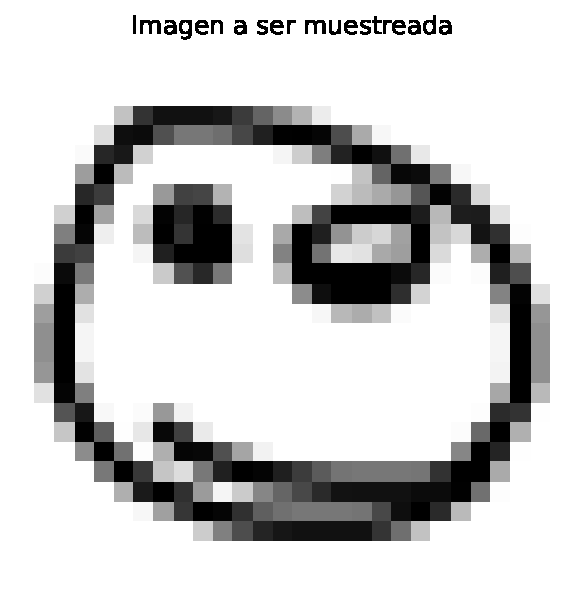
\includegraphics[height=6cm]{img/distr_draw/face_distrib.pdf}
        \caption{Imagen de una cara.}
        \label{fig:face-distrib}
    \end{subfigure}
    \hfill
    \begin{subfigure}[b]{0.45\textwidth}
        \centering
        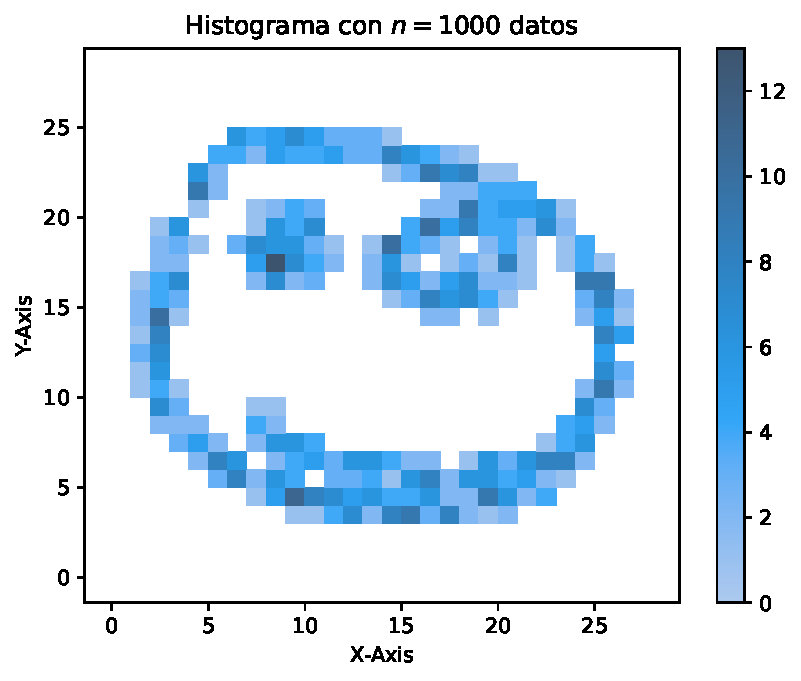
\includegraphics[height=6cm]{img/distr_draw/face_hist.pdf}
        \caption{Histograma de $n=1000$ muestras.}
        \label{fig:face-hist}
    \end{subfigure}
    \caption{Ejemplo de una distribución que proviene de una imagen. Elaboración propia.}
    \label{fig:face-example}
\end{figure}

\subsection{Implementación del Algoritmo}\label{ssec:implementacion-algoritmo}  % MARK: - Implementación del Algoritmo

Dado que el Algoritmo~\ref{alg:sgdw-clasico} está diseñado para medidas absolutamente continuas, se reinterpreta este algoritmo para que se pueda trabajar con medidas discretas. Para ello, se destaca que la Definición~\ref{def:sgdw} se puede reinterpretar como la $\eta_k$-interpolación geodésica entre las medidas $\mu_k$ y $\tilde \mu_k$, mientras que la Definición~\ref{def:bsgdw} se puede reinterpretar como el baricentro de las medidas $\qty( \mu_k, \tilde\mu_k^{(1)}, \dots, \tilde\mu_k^{(S_k)} )$ con pesos $\qty(1-\eta_k, \frac{\eta_k}{S_k}, \dots, \frac{\eta_k}{S_k}) \in \Simplex[S_k+1]$. De este modo, el Algoritmo~\ref{alg:sgdw-clasico} se extiende de la siguiente manera:
\begin{algorithm}[H]
    \caption{SGDW General}
    \label{alg:sgdw-general}
    \begin{algorithmic}[1]
        \Require Acceso a las muestras de $\Gamma(\dd \mu) \in \ProbSpace[\ProbSpace]$, un esquema de paso $(\eta_k)_k \in [0, 1]^\N$ y un esquema de paso $(S_k)_k \in \N^\N$.
        \State{$k\gets0$}
        \State{Muestrear $\mu_0 \sim \Gamma$}
        \Repeat
        \State{Muestrear $\tilde \mu_k^{(1)}, \dots, \tilde \mu_k^{(S_k)} \simiid \Gamma$}
        \State{$\gamma\gets\qty(1-\eta_k, \frac{\eta_k}{S_k}, \dots, \frac{\eta_k}{S_k})$}
        \State Definir $\mu_k$ como el baricentro de $\qty( \mu_k, \tilde\mu_k^{(1)}, \dots, \tilde\mu_k^{(S_k)} )$ con pesos $\gamma$.
        \State{$k\gets k+1$}
        \Until{un criterio de detención ha sido alcanzado.}
        \State\Return $\mu_k$
    \end{algorithmic}
\end{algorithm}

Cabe destacar que en el Algoritmo~\ref{alg:sgdw-general} se mantiene la versión de la secuencia por lotes. Esto es para mantener una mayor generalidad, pues el caso original del Algoritmo~\ref{alg:sgdw-clasico} se recupera considerando $S_k=1,\ \forall k\in\N$.

Como se está trabajando con imágenes, se puede aprovechar su estructura para calcular una estimación de los baricentros de manera más eficiente, utilizando el algoritmo de Baricentros de Wasserstein Convolucionales \cite{solomon2015convolutional} o su versión Insesgada (\textit{Debiased} en inglés) \cite{janati2020debiased}. Sin embargo, el Algoritmo~\ref{alg:sgdw-general} es lo suficientemente general para ser aplicado a cualquier medida discreta, utilizando por ejemplo, la estimación del algoritmo de Sinkhorn \cite{cuturi2013sinkhorn}.

Todos estos métodos de cálculo de baricentros se implementan de manera eficiente utilizando la librería de \textit{Python Optimal Transport} (POT) \cite{flamary2021pot}, donde además esta librería admite la paralelización de los cálculos por medio de la computación de Propósito General en Unidades de Procesamiento Gráfico (GPGPU por sus siglas en inglés) \cite{owens2008gpu}. En la implementación, se mantienen las versiones tanto para imágenes, como para medidas discretas genéricas, en función de obtener una mayor generalidad y versatilidad.

\subsubsection{Medidas de Probabilidad}\label{sssec:medidas}  % MARK: - Medidas

Se considera una medida de referencia $\Prob_X \in \ProbSpace[\ProbSpace[\cX]]$ que corresponde a una forma ``idealizada'' del conjunto de datos \textit{Quick, Draw!} \cite{jongejan2016quick}. Esto es, si es que se tuviera un acceso ilimitado a muestras parecidas a este conjunto de datos, entonces este sería $\Prob_X$. Se desea calcular el baricentro de esta medida, utilizando el Algoritmo~\ref{alg:sgdw-general}.

Para ello, se consideran dos aproximaciones de $\Prob_X$. La primera, es la empírica:
\begin{equation}\label{eq:medida-empirica-quick-draw}
    \hat \Prob_X = \frac{1}{N} \sum_{i=1}^{N} \delta_{\mu_i},
\end{equation}
donde $\left\{ \mu_i \right\}_{i=1}^{N} \subseteq \ProbSpace[\cX] $ es el conjunto de datos obtenido de la Sección~\ref{ssec:preparacion-dataset}, y $N$ es el tamaño del conjunto de datos. La segunda, es la medida generada por la WGAN $G_\theta : \cZ \to \ProbSpace[\cX]$, entrenada como se explica en el Capítulo~\ref{chap:WAE-WGAN}:
\begin{equation}
    \tilde \Prob_X
    = \pf{G_\theta} \Prob_Z
\end{equation}
donde $\Prob_Z$ es la medida del espacio latente (en este caso, una distribución normal estándar). En la Figura~\ref{fig:sample-empirico} se presentan muestras de la medida empírica $\hat\Prob_X$ y en la Figura~\ref{fig:sample-gan} de la medida generadora $\tilde\Prob_X$.

\begin{figure}[htbp]
    \centering
    \begin{subfigure}[b]{0.45\textwidth}
        \centering
        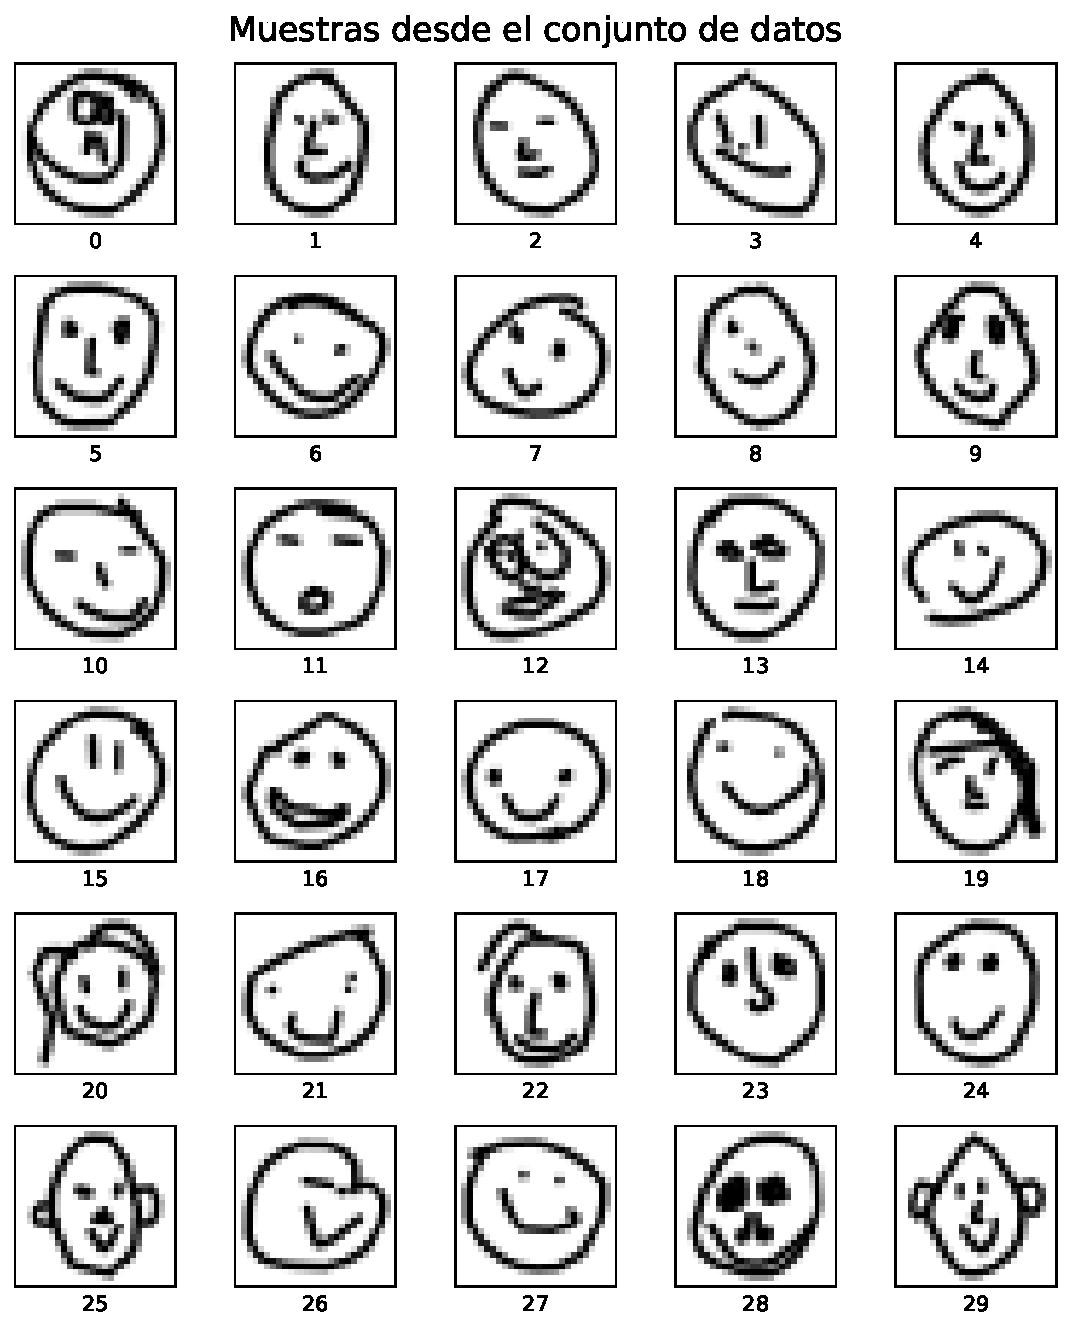
\includegraphics[width=\textwidth]{img/distr-sampler/UniformDiscreteSampler-6x5.pdf}
        \caption{Muestras desde la medida empírica $\hat\Prob_X$}
        \label{fig:sample-empirico}
    \end{subfigure}
    \hfill
    \begin{subfigure}[b]{0.45\textwidth}
        \centering
        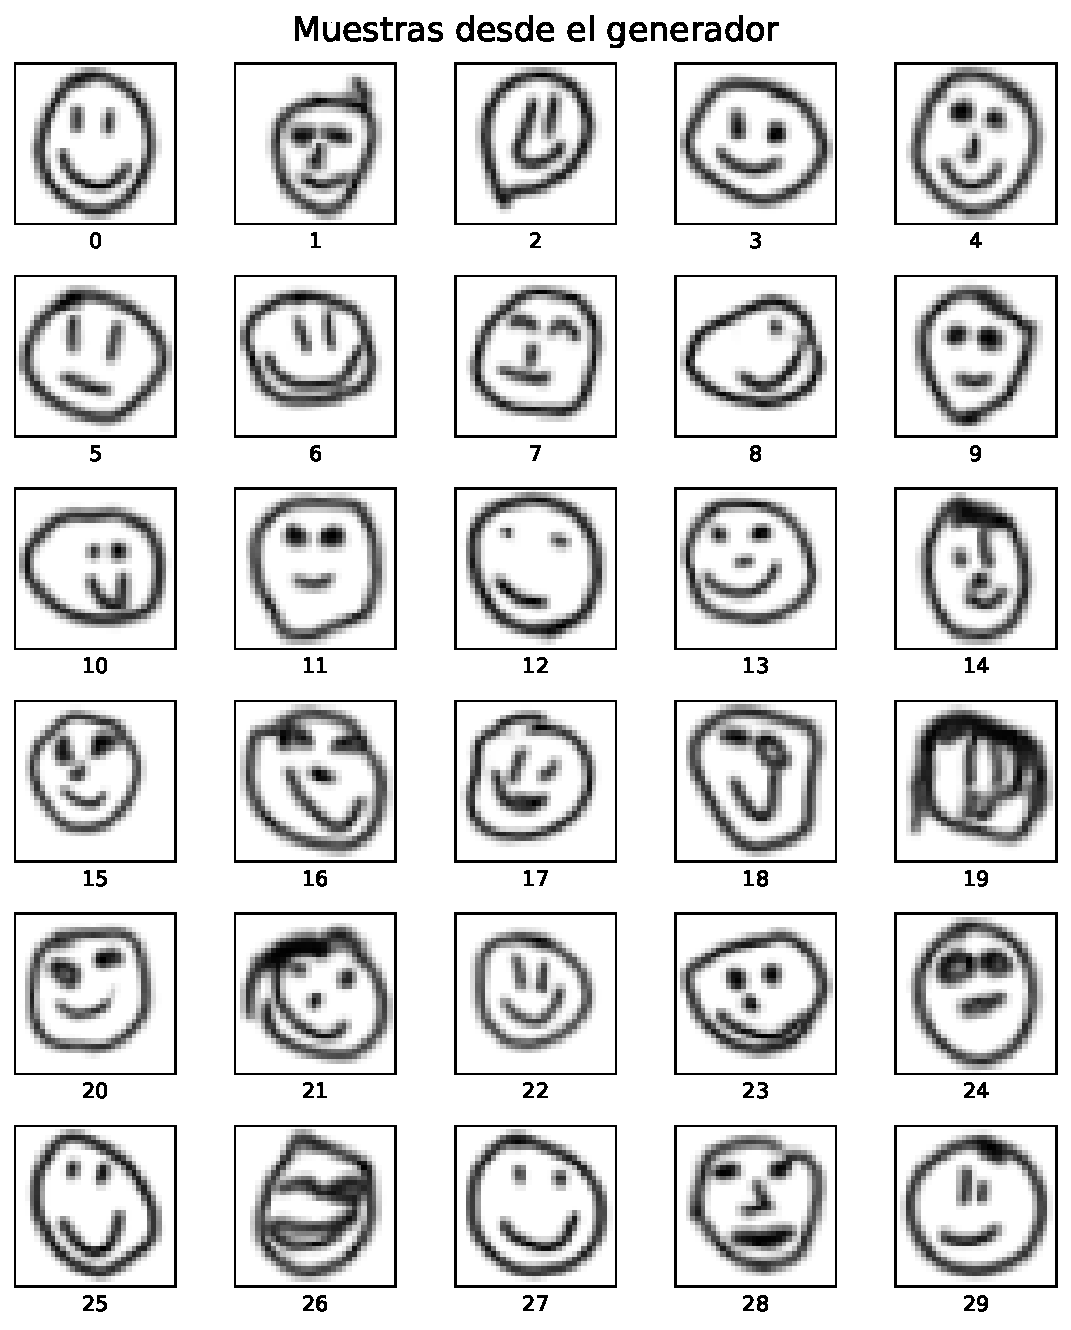
\includegraphics[width=\textwidth]{img/distr-sampler/GeneratorDistribSampler-6x5.pdf}
        \caption{Muestras desde la medida generadora $\tilde\Prob_X$}
        \label{fig:sample-gan}
    \end{subfigure}
    \caption{Muestras de las medidas $\hat\Prob_X$ y $\tilde\Prob_X$ para el conjunto de datos \textit{Quick, Draw}.}
    \label{fig:sample}
\end{figure}


\subsubsection{Experimentos}\label{sssec:experimentos-sgdw}  % MARK: - Experimentos

Como $\hat \Prob_X$ y $\tilde \Prob_X$ son estimaciones de la medida de referencia $\Prob_X$, se espera que el baricentro de población de estas medidas sean similares entre sí. Por este motivo, se calculan los baricentros utilizando el Algoritmo~\ref{alg:sgdw-general} para ambas medidas, y se comparan los resultados obtenidos.

Para el algoritmo, se utiliza el siguiente esquema de paso:
\begin{equation}\label{eq:esquema-paso}
    \eta_k = \frac{a}{(b^{1/c} + k)^c},\quad \forall k \in \N.
\end{equation}
Este esquema es una reparametrización del que se presenta en \cite[Secc.~2]{welling2011bayesian}. Se puede demostrar que, cuando $a > 1$, $b > 0$ y $0.5 < c \leq 1$, entonces $(\eta_k)_{k}$ cumple con las siguientes condiciones:
\begin{align}
    \sum_{k=0}^{\infty} \eta_k   & = \infty, &
    \sum_{k=0}^{\infty} \eta_k^2 & < \infty.
\end{align}
Estas dos condiciones son usuales en la optimización convexa, pues garantizan la convergencia del algoritmo. En los experimentos se utilizan $a = 3$, $b = 3,01$ y $c = 0,501$. Se escogen estos parámetros para que se cumplan las siguientes condiciones:
\begin{equation}
    \forall k\in\N \colon \eta_k\in[0, 1]\qquad \text{y} \qquad \eta_0 = \frac{a}{b} \lesssim 1.
\end{equation}

Además, para estas dos medidas, se consideran dos esquemas para el número de lotes $S_k$: uno simple $S_k = 1$, que correspondería al caso original, y otro más complejo $S_k = 5$, para observar el efecto de una convergencia más rápida.

Para la estimación del baricentro de Wasserstein en el paso 6 del Algoritmo~\ref{alg:sgdw-general}, se utiliza el método del Baricentro de Wasserstein Convolucional Insesgado \cite{janati2020debiased}. Para mayor detalle de los parámetros utilizados, se puede consultar el Anexo~\ref{sec:compl-sgdw-params-adicional}.

Los resultados de las iteraciones se presentan a continuación:
\begin{figure}[htbp]
    \centering
    \begin{subfigure}[b]{0.45\textwidth}
        \centering
        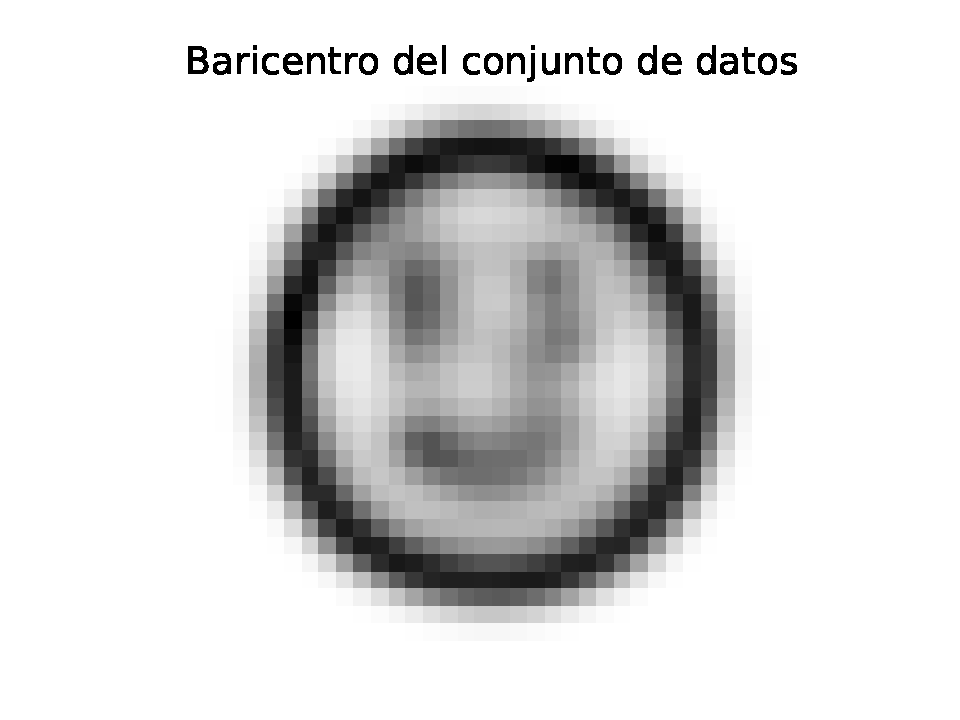
\includegraphics[width=0.75\textwidth]{img/barycenters/bar-DS.pdf}
        \caption{Baricentro de la medida empírica $\hat\Prob_X$.}
        \label{fig:bar-DS}
    \end{subfigure}
    \hfill
    \begin{subfigure}[b]{0.45\textwidth}
        \centering
        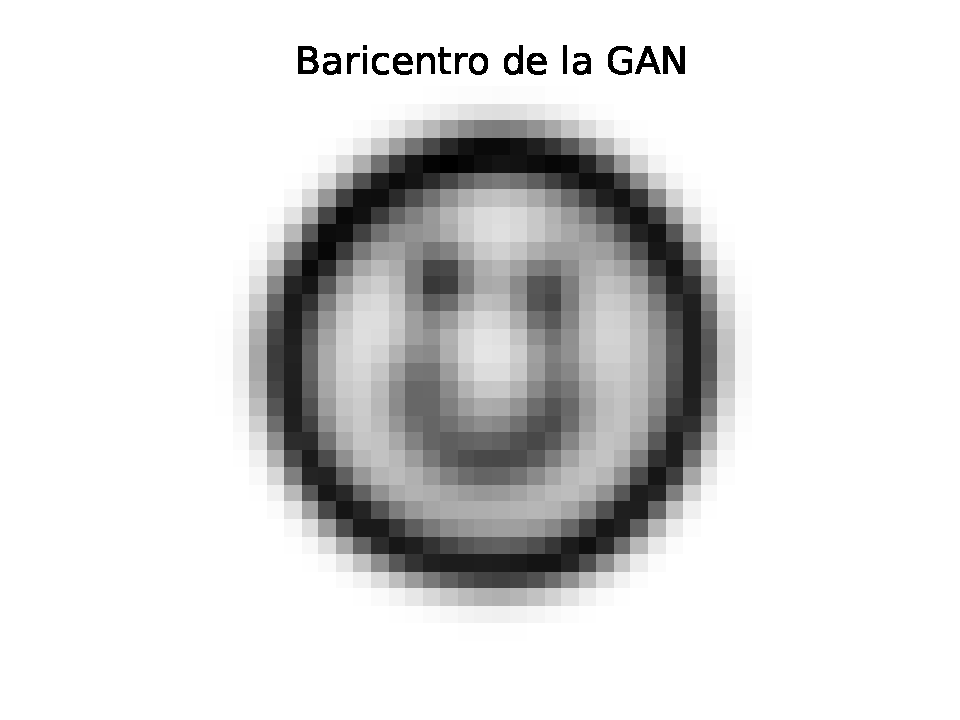
\includegraphics[width=0.75\textwidth]{img/barycenters/bar-GAN.pdf}
        \caption{Baricentro de la medida generadora $\tilde\Prob_X$.}
        \label{fig:bar-GAN}
    \end{subfigure}
    \newline
    \begin{subfigure}[b]{0.45\textwidth}
        \centering
        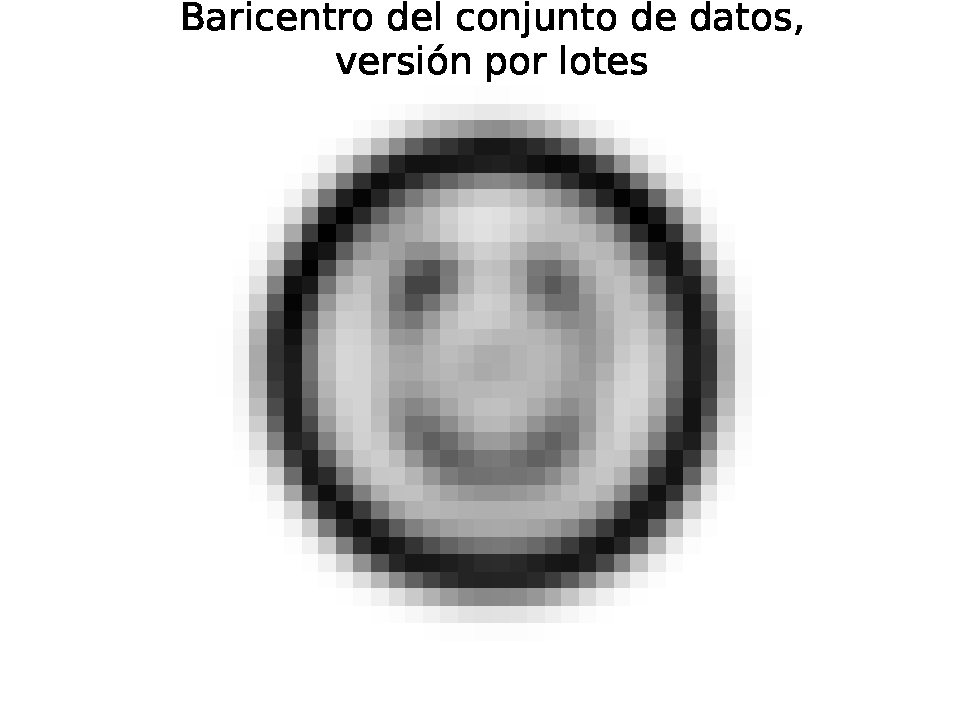
\includegraphics[width=0.75\textwidth]{img/barycenters/batch-bar-DS.pdf}
        \caption{Baricentro de la medida empírica $\hat\Prob_X$, versión~por lotes.}
        \label{fig:batch-bar-DS}
    \end{subfigure}
    \hfill
    \begin{subfigure}[b]{0.45\textwidth}
        \centering
        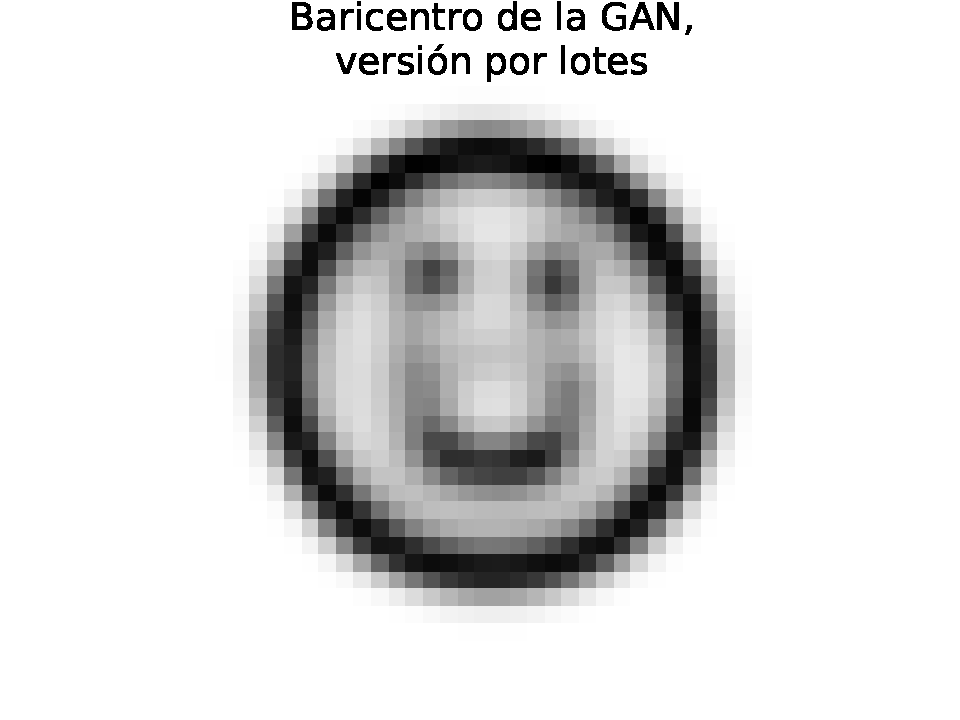
\includegraphics[width=0.75\textwidth]{img/barycenters/batch-bar-GAN.pdf}
        \caption{Baricentro de la medida generadora $\tilde\Prob_X$, versión por lotes.}
        \label{fig:batch-bar-GAN}
    \end{subfigure}
    \caption{Baricentros de población de las medidas $\hat\Prob_X$ y $\tilde\Prob_X$ para el conjunto de datos \textit{Quick, Draw}, utilizando $S_k=1$ y $S_k=5$.}
    \label{fig:barycenters}
\end{figure}

En las Figuras~\ref{fig:iters-DS}, \ref{fig:iters-GAN}, \ref{fig:batch-iters-DS} y \ref{fig:batch-iters-GAN} se presentan las primeras y últimas iteraciones para el cálculo de los baricentros anteriormente mencionados.


% MARK: - Empirica
\begin{figure}[H]
    \centering
    \begin{subfigure}[b]{0.75\textwidth}
        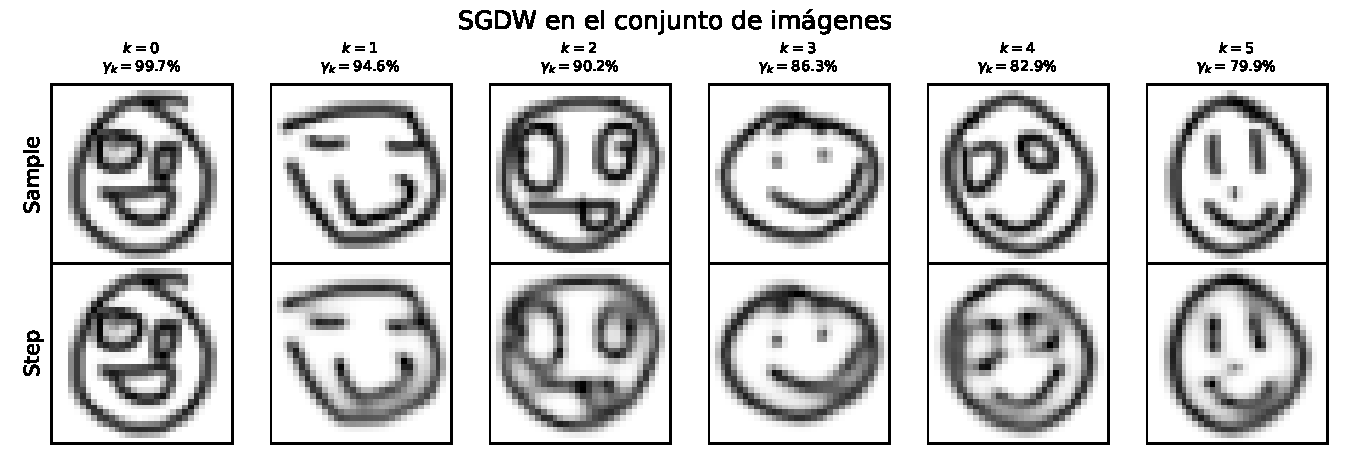
\includegraphics[width=\textwidth]{img/sgdw-iters/first-iters-DS.pdf}
        \caption{Primeras iteraciones.}
        \label{fig:first-iters-DS}
    \end{subfigure}
    \begin{subfigure}[b]{0.75\textwidth}
        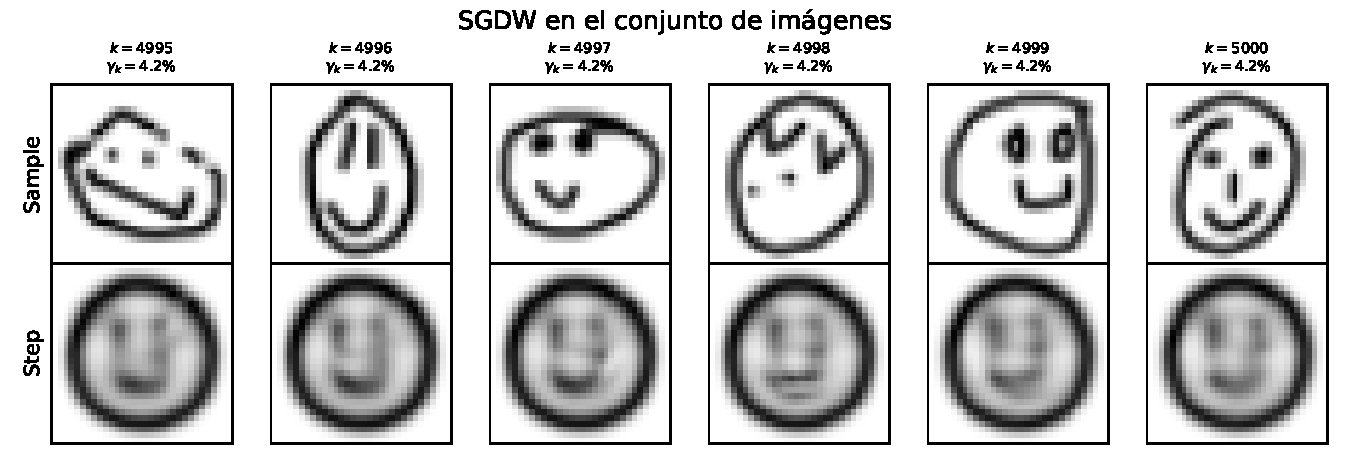
\includegraphics[width=\textwidth]{img/sgdw-iters/last-iters-DS.pdf}
        \caption{Últimas iteraciones.}
        \label{fig:last-iters-DS}
    \end{subfigure}
    \caption{Iteraciones del cálculo del baricentro de $\hat\Prob_X$.}
    \label{fig:iters-DS}
\end{figure}

% MARK: - GAN
\begin{figure}[H]
    \centering
    \begin{subfigure}[b]{0.75\textwidth}
        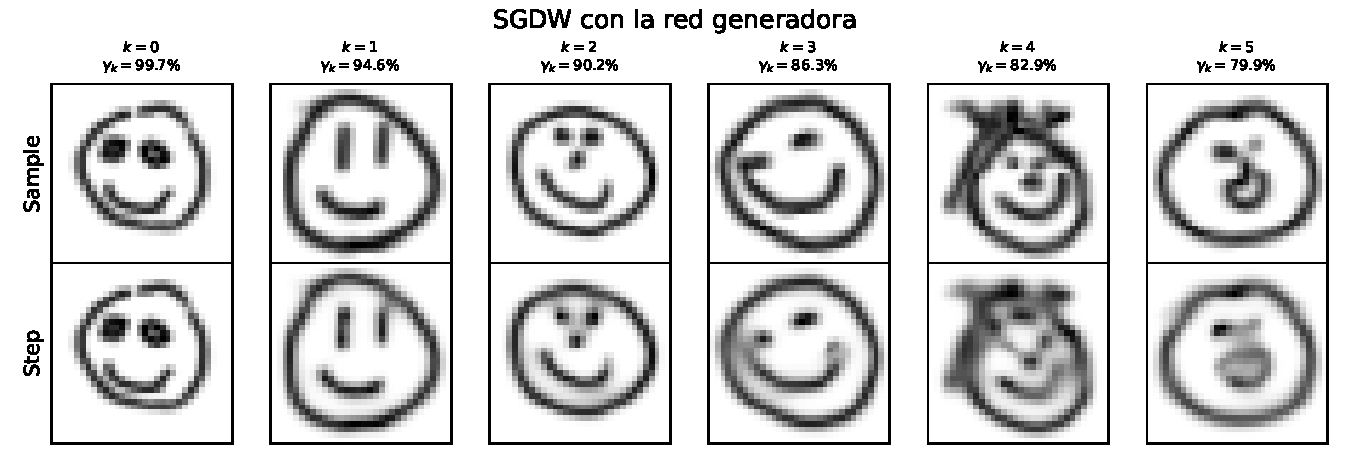
\includegraphics[width=\textwidth]{img/sgdw-iters/first-iters-GAN.pdf}
        \caption{Primeras iteraciones.}
        \label{fig:first-iters-GAN}
    \end{subfigure}
    \begin{subfigure}[b]{0.75\textwidth}
        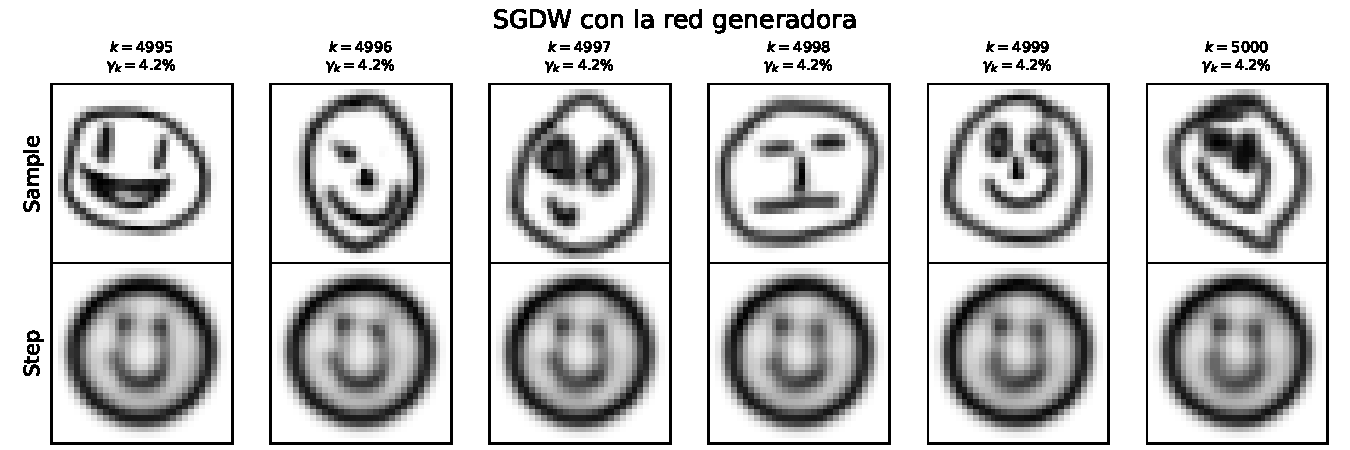
\includegraphics[width=\textwidth]{img/sgdw-iters/last-iters-GAN.pdf}
        \caption{Últimas iteraciones.}
        \label{fig:last-iters-GAN}
    \end{subfigure}
    \caption{Iteraciones del cálculo del baricentro de $\tilde\Prob_X$.}
    \label{fig:iters-GAN}
\end{figure}

% MARK: - Empirica Batched
\begin{figure}[H]
    \centering
    \begin{subfigure}[b]{0.75\textwidth}
        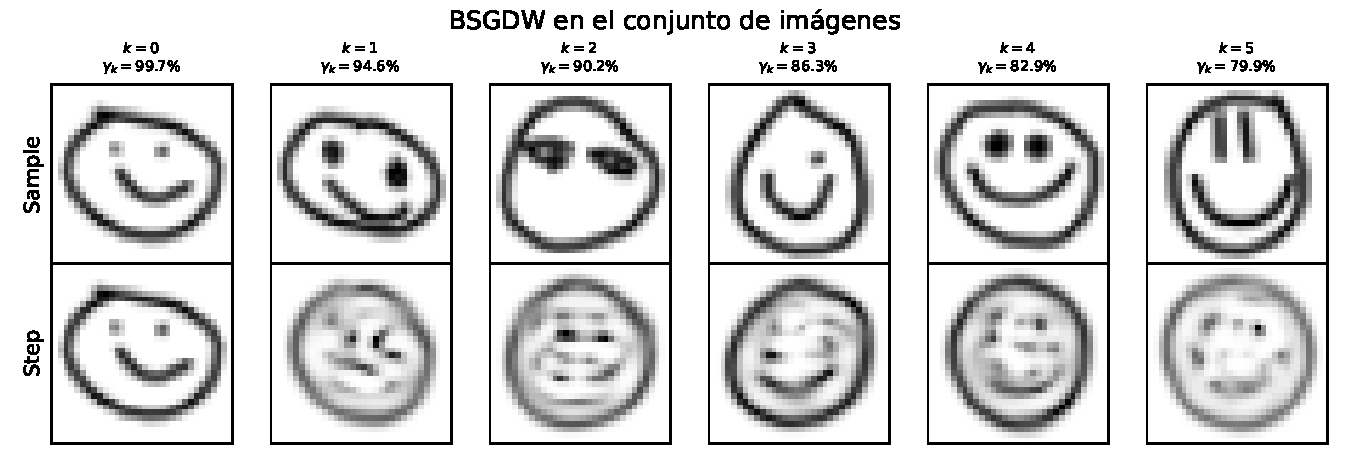
\includegraphics[width=\textwidth]{img/sgdw-iters/batch-first-iters-DS.pdf}
        \caption{Primeras iteraciones.}
        \label{fig:batch-first-iters-DS}
    \end{subfigure}
    \begin{subfigure}[b]{0.75\textwidth}
        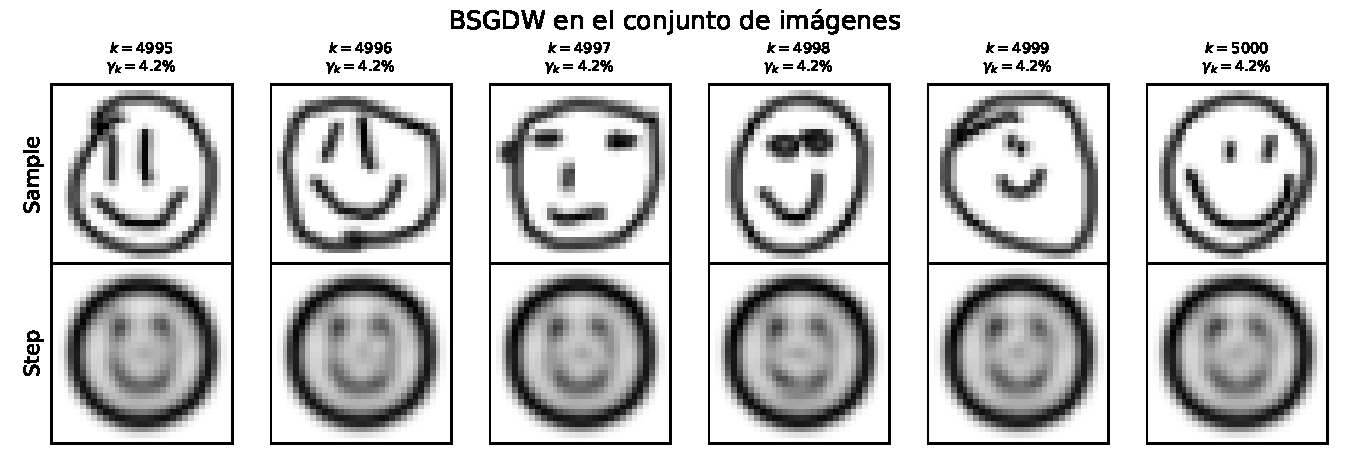
\includegraphics[width=\textwidth]{img/sgdw-iters/batch-last-iters-DS.pdf}
        \caption{Últimas iteraciones.}
        \label{fig:batch-last-iters-DS}
    \end{subfigure}
    \caption{Iteraciones del cálculo del baricentro de $\hat\Prob_X$ en su versión por lotes.}
    \label{fig:batch-iters-DS}
\end{figure}

% MARK: - GAN Batched
\begin{figure}[H]
    \centering
    \begin{subfigure}[b]{0.75\textwidth}
        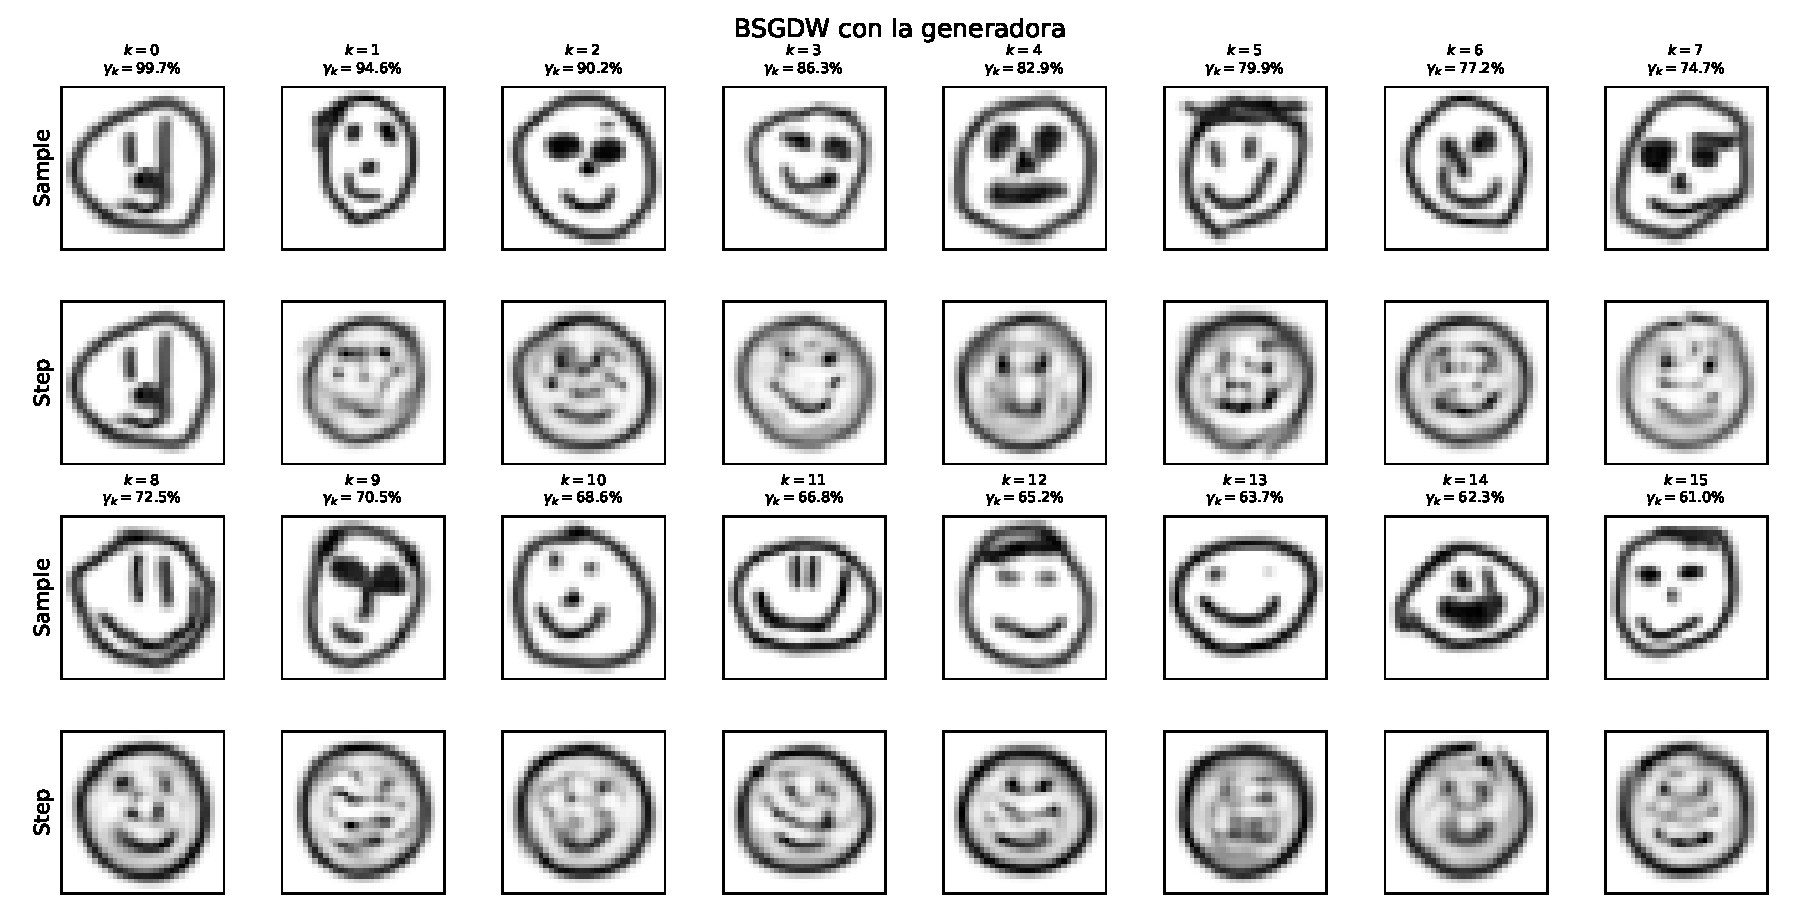
\includegraphics[width=\textwidth]{img/sgdw-iters/batch-first-iters-GAN.pdf}
        \caption{Primeras iteraciones.}
        \label{fig:batch-first-iters-GAN}
    \end{subfigure}
    \begin{subfigure}[b]{0.75\textwidth}
        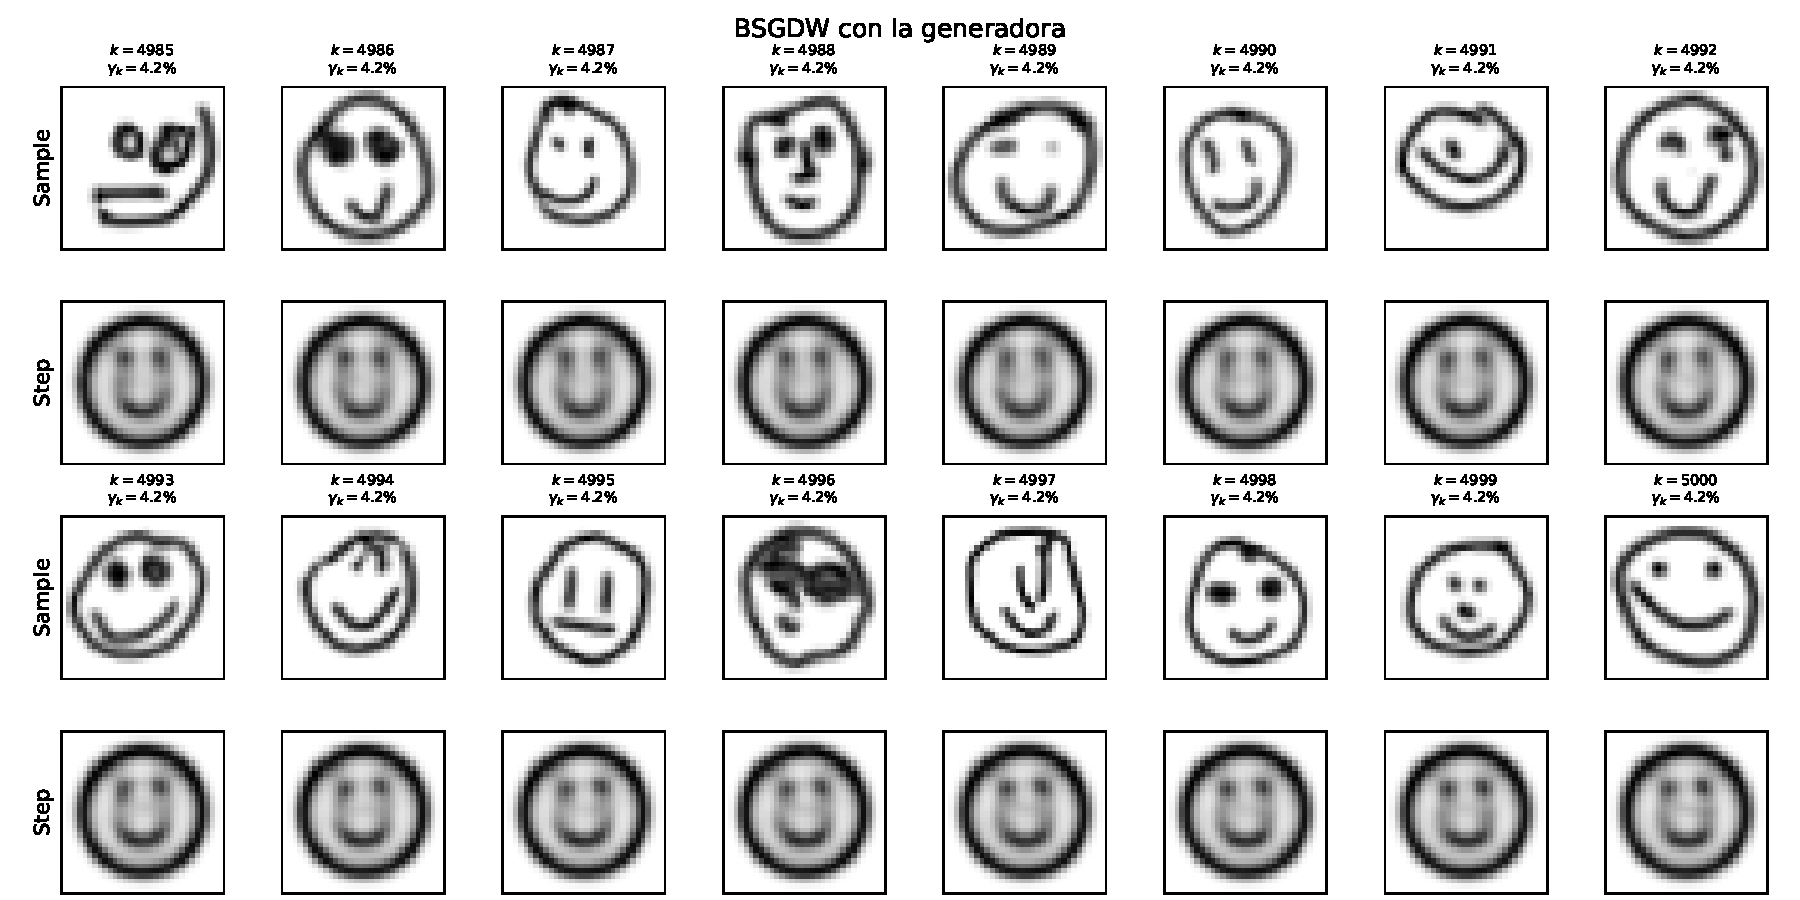
\includegraphics[width=\textwidth]{img/sgdw-iters/batch-last-iters-GAN.pdf}
        \caption{Últimas iteraciones.}
        \label{fig:batch-last-iters-GAN}
    \end{subfigure}
    \caption{Iteraciones del cálculo del baricentro de $\tilde\Prob_X$ en su versión por lotes.}
    \label{fig:batch-iters-GAN}
\end{figure}

Se puede notar cómo en las primeras iteraciones de las Figuras~\ref{fig:first-iters-DS} y \ref{fig:first-iters-GAN}, la estimación del baricentro varía mucho entre una iteración y otra, debido al esquema de paso utilizado. Sin embargo, a medida que se avanza en las iteraciones, la estimación del baricentro se estabiliza. Además, se puede observar en las Figuras~\ref{fig:batch-first-iters-DS} y \ref{fig:batch-first-iters-GAN} que el método por lotes provee imágenes más difusas en las primeras iteraciones, debido a la mayor cantidad de muestras utilizadas en el cálculo del baricentro. No obstante, proporciona resultados muy similares a su versión simplificada en un menor tiempo de ejecución.


% En el Anexo~\ref{sec:compl-sgdw-iters} se presentan las primeras y últimas iteraciones del cálculo de los baricentros, tanto para la medida empírica $\hat\Prob_X$ como para la medida generadora $\tilde\Prob_X$.












% \subsection{Resultados y Discusión}\label{ssec:sgdw-resultados-discusion}  % MARK: -- Resultados y Discusión

% \FM[inline]{En esta sección se podría incluir el cálculo de un baricentro, tanto del dataset como de la GAN}

\subsection{Conclusiones}\label{ssec:sgdw-conclusiones}  % MARK: -- Conclusiones

Se puede observar que los baricentros obtenidos para los cuatro experimentos (los obtenidos en la Figura~\ref{fig:barycenters}) son muy similares entre sí, comprobando la hipótesis inicial. Es lo esperable, pues tanto $\hat\Prob_X$ como $\tilde\Prob_X$ son aproximaciones de la medida de referencia $\Prob_X$.  Además, a partir de las Figuras~\ref{fig:batch-first-iters-DS} y \ref{fig:batch-first-iters-GAN} se puede observar que efectivamente el método por lotes converge más rápido que el método original, resultando en baricentros muy similares a su versión simplificada.

